\documentclass{article}
\usepackage[utf8]{inputenc}
\usepackage{graphicx}
\usepackage[top=1in,bottom=1in,left=1in,right=1in]{geometry}
\setlength{\parindent}{0pt} 


\title{PS6-Onishi}
\author{Saryu Onishi}
\date{March 2023}

\begin{document}

\maketitle
\section{The data set}
For this problem set, I used the same R package as the PS5 to scrape data from my own Strava page. I then extracted only the data I wanted. Specifically, I filtered the data by latitude and longitude to display my Strava activities in and around the Norman area.

I decided not to transform the data too much beyond this since the data table was not the primary purpose of this assignment. However, if I was to present the table, I would use the 'select' command to remove columns that may not be useful to construct the visualizations. I would also reorganize the table to display the activity ID and activity title at the leftmost columns.

\section{viz 1: heat map}
The first visualisation is a general heat map of all activities in the specified area. In this case, the specified area was the Norman area. 
This shows us how concentrated the activities are in a specific region.
\begin{figure}[h]
\centering
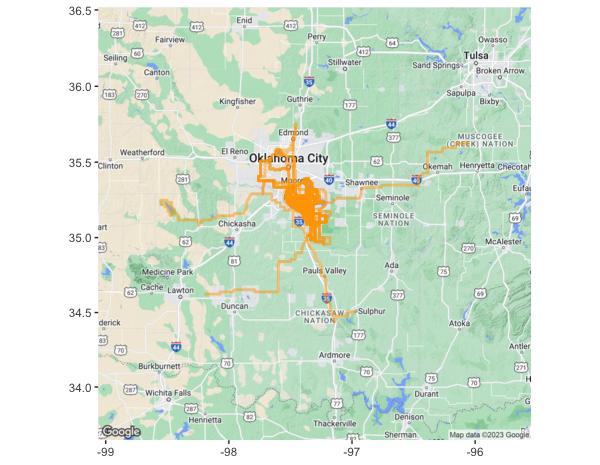
\includegraphics[width=0.5\textwidth]{PS6a_Onishi.png}
\caption{Activity Heatmap}
\end{figure}

\section{viz 2: elevation chart}
Next, I isolated one particular activity and using its activity ID and decided to visualize the elevation data. This is a course profile that shows the elevation data as a line/area chart. Typically, you would see this is the sort of chart during a race presentation. 
Although this type of chart is informative, we can see a few limitations. Using this kind of chart would involve cross-referencing a map with distance markers, which can be a hassle, and an extra step that could be easily avoided.
\begin{figure}[h]
\centering
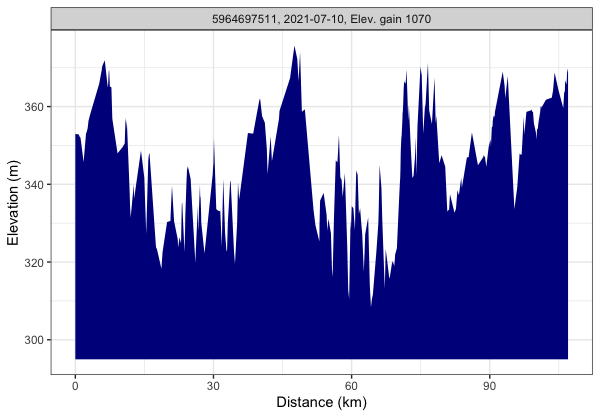
\includegraphics[width=0.5\textwidth]{PS6b_Onishi.png}
\caption{Elevation chart}
\end{figure}

\section{viz 3: elevation overlaid on a map}
To improve upon the chart above, we can combine ideas from the first map, with the second chart. By overlaying the elevation data on top of a map, we can now eliminate a step for our audience. It is easier to piure what the elevation range is (due to the legend), and where the changes are exactly.
\begin{figure}[h]
\centering
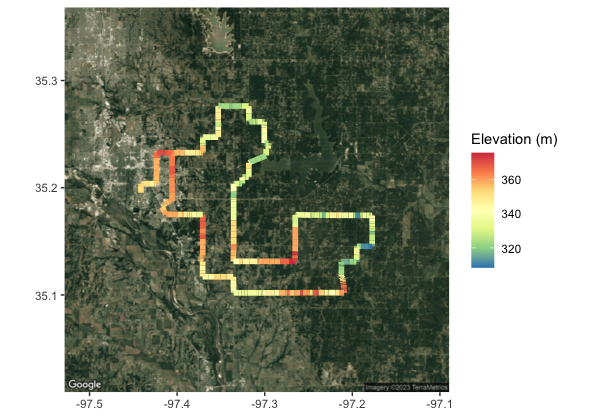
\includegraphics[width=0.5\textwidth]{PS6c_Onishi.png}
\caption{Elevation map}
\end{figure}

\section{Conclusion}
As a concluding note, I thought that the rStrava package was helpful in generating these unique ways of visualizing activity data. However, I think there is a big limitation because only data from one individual can be used, as each request has to be authenticated by the person who owns the account.
With this said, its capacity to overlay data onto maps is a great way to visualize different aspects of activity data.


\end{document}

